\chapter{Sequence-Based Predictions}
In the following chapter we touch on some important and useful prediction methods that
have only this in common: they take as input the \textit{aminoacid sequence}. We will see
that you can do a lot of things with sequences alone. 
The first distinction we need to make is between:
\begin{itemize}
    \item methods that deal with a single protein. Typically, you search for
    structural features, or protein-protein interaction motifs;
    \item comparative methods ($\geq 2$ proteins). Typically, you use them to investigate the
    evolutionary story of proteins.
\end{itemize}

\section{Practical checklist}
There are some tecnhical aspects that you might overlook when you download your sequence from UniProt. 
It is really important that you check these things, because they may screw your project completely.

\begin{enumerate}
    \item  \textbf{Is the sequence correct?} You cannot know yet how to check this, we will have a dedicated lecture on that. For the moment, keep in mind that it is a possible issue;
    \item \textbf{Is the sequence corresponding to the matured, active protein?} There is some biology that you need to know. First, proteins are often synthetized with an 
    extra string of aminoacid at the beginning, called \textit{signal peptide}. This acts like a "zip code" and instructs the cell about where the protein should be sent (for example, to mythocondria, to the endoplasmic reticulum, or outside the cell).
    Once the protein arrives at its correct location, the signal peptide is cleaved off. You should check that your sequence does not contain the initial signal peptide before you start analyzing it. Second,
    beware that some proteins are synthetized in an inactive form (\textit{zymogens}), because they are potentially harmful and only need to be activated in specific environments. 
    For example, the enzymes that demolish proteins (called \textit{proteases}, for example \textit{trypsin} or\textit{pepsin}) are in the inactive form by default, and only axctivated in the stomach.
    Otherwise, they would eat the cell! So, always check that you are using the active form of the protein.
    \item \textbf{Is the sequence a wild type or a mutant?} With "wild type" we refer to the version of the protein that typically occurs in nature. A "mutant" is a protein that has undergone
    some modification (mismatch, insertion, deletion).
    \item \textbf{Is the protein post-translationally modified (PTM)?} 
    \item \textbf{Is the protein from the right organism?}
\end{enumerate}

Also, beware that sometimes you will find "mysterious" letters in the sequences you download. This is due to the fact
that crystallography data can be "blurry" and the scientists may not be able to know the identity of all residues. They use ambiguity codes to fill the gaps:

\begin{itemize}
\item X: Any amino acid (Unknown).
\item Z: Either Glutamic acid (E) or Glutamine (Q). They look very similar in certain chemical tests.
\item B: Either Aspartic acid (D) or Asparagine (N).
\end{itemize}

\section{Sequence-based prediction on a single protein}
In this section we explore the ways in which you can exploit a protein sequence
to say something aobut its structural features or other things you might be interested in,
for exaple protein-protein interaction motifs, or disease association.

Before starting, it is important to stress that you should never overlook the single-protein sequence based predictions.
These methods are fast ($\mathcal{O}(N)$), effective on a lot of tasks, and also much less dataset-dependent than methods
like AlphaFold. 

AlphaFold or BLAST and similar are "evolutionary methods" in the sense that they only work if the protein has "relatives" already sitting in a database.
If you discover a completely unique protein (an "orphan" protein), evolutionary methods will fail. 
Physico-chemical methods will still work because they only care about the amino acids in front of them. 


\subsection{Using amino-acid physio-chemical properties}
Open ProtScale: \url{https://web.expasy.org/protscale/}. As a walk-through example, we will analyze human (pig) myoglobin.

\begin{verbatim}
    PIG MIOGLOBIN: 
PDB 1PMB
Uniprot: P02189 · MYG_PIG
MGLSDGEWQLVLNVWGKVEADVAGHGQEVLIRLFKGHPETLEKFDKFKHLKSEDEMKASEDLKKH
GNTVLTALGGILKKKGHHEAELTPLAQSHATKHKIPVKYLEFISEAIIQVLQSKHPGDFGADAQG
AMSKALELFRNDMAAKYKELGFQG
\end{verbatim}

We can get a fairly good intuition of the structure that the protein will take on,
just by interpreting the outputs of some simple scales. 

Let's start by considering the \textbf{Kylie-Doolittle (KD) hydrophaty scale}. In this scale, \textbf{positive values indicate hydrophobicity}. This is not the only hydropathy scale: there are dozens!
And they are all based on slightly different experimental methods, therefore it is important to \textit{compare} the results you obtain with a scale to those you obtain 
with other scales, to verify that they are \textit{robust}. 

The mosty common method of measuring amino acid hydrophobicity is partitioning between two immiscible liquid phases:
\begin{enumerate}
    \item take a two-phase liquid system that doesn't mix, like Water (polar) and Octanol (non-polar).
    \item  add a specific amino acid to the mixture
    \item shake and let the layers separate again
    \item measure the concentration of the amino acid in each layer.
\end{enumerate} 
The partition coefficient is the ratio of aminoacid concentrations in the two solvents.


\begin{figure}[h!]
    \centering
    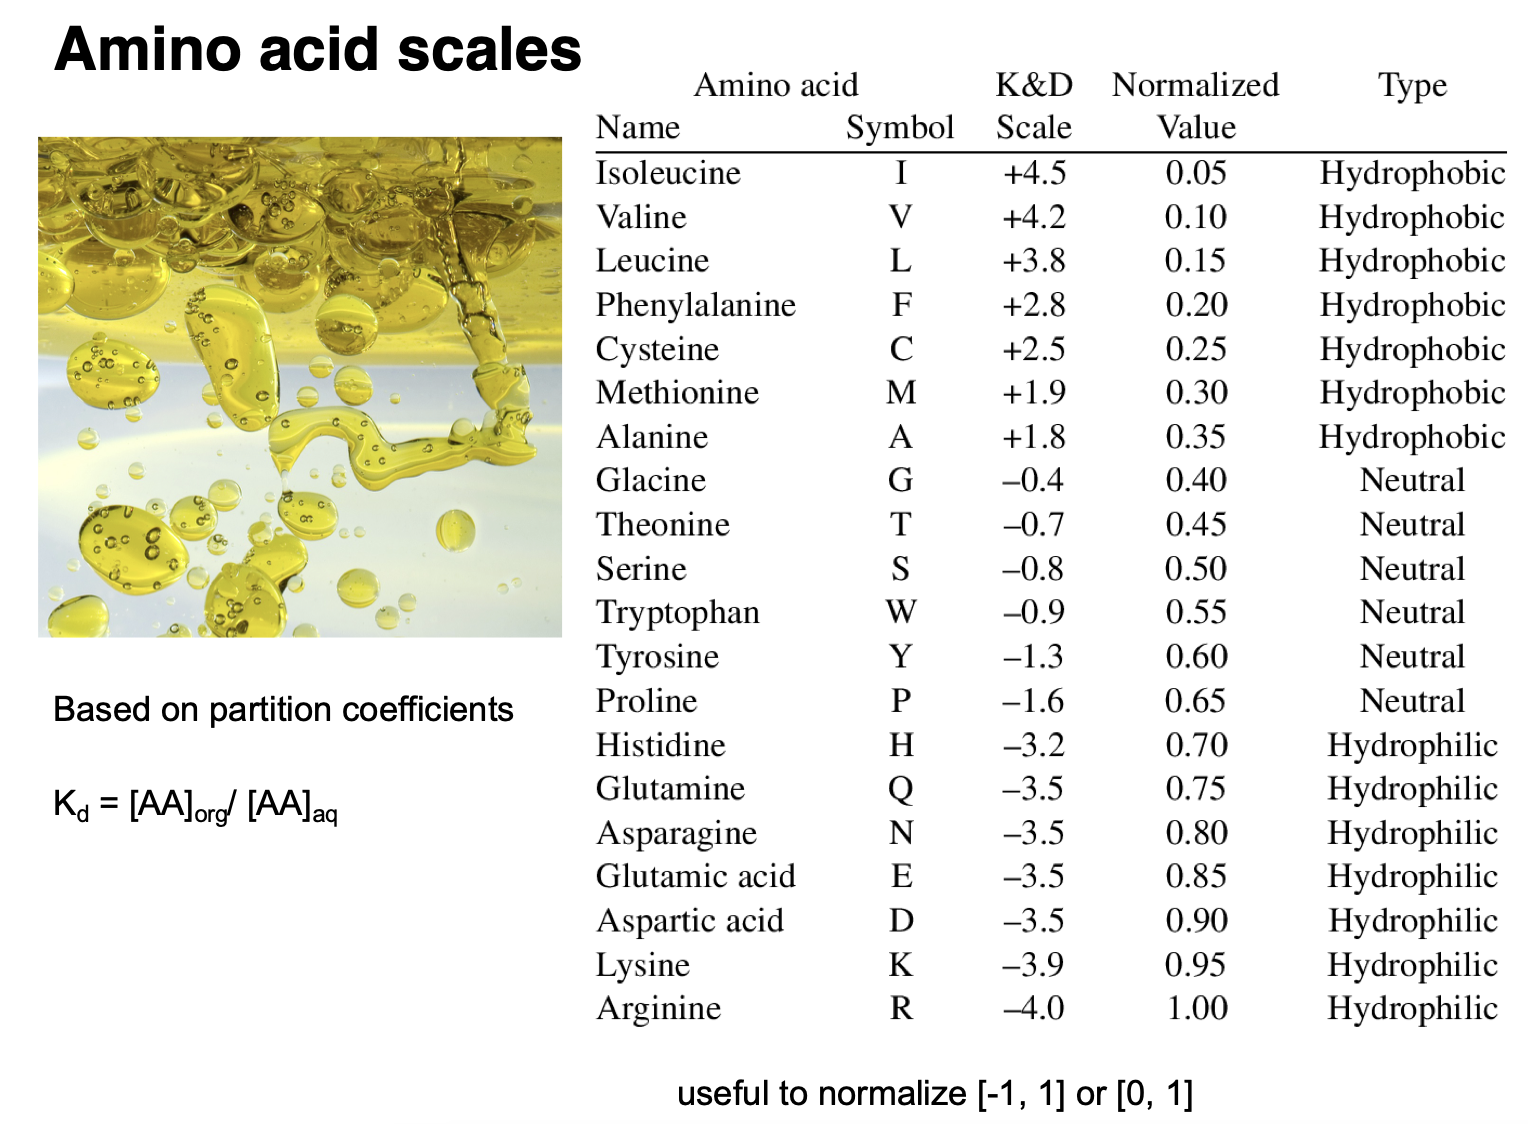
\includegraphics[width=\linewidth]{slides/sequence_based_predictions/hydrophob_scale.png}
    \caption{}
\end{figure}




First of all, you need to choose the window size. The optimal choice depends on which feature you are investigating, if its \textit{local} or \textit{global}. For detection
of secondary structure elements, like $\alpha$-helices, you need a medium size ($\sim 9$). Instead, if you aim to detect functional motifs,
that are usually short, you will choose a smaller window size.
\begin{figure}[h!]
    \centering
    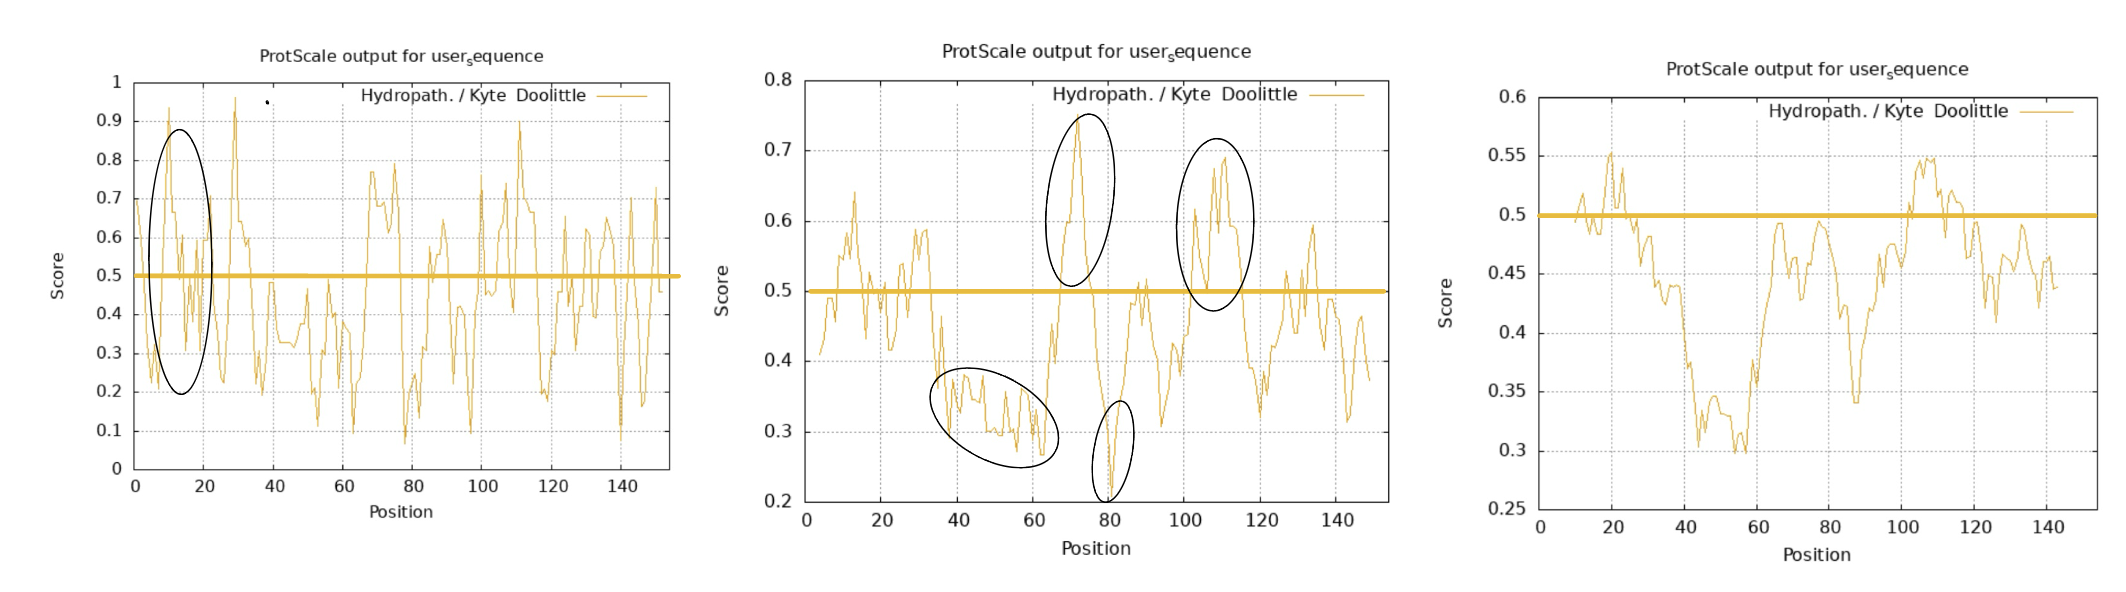
\includegraphics[width=\linewidth]{slides/sequence_based_predictions/different_windows.png}
    \caption{From left to right, window sizes of $3$, $9$, and $21$. \textbf{Center}: medium window size. We can use this to get a grasp of
    how we expect the protein structure to be. For instance, we see two highly hidrophobic patches. We can reasonably expect that they correspond to
    the protein core. Also, we see some highly hydrophilic regions: these could be loops or coils that are highly exposed to the solvent and are connecting 
    some secondary structures like $\alpha$- helices. Helices are expected to correspond to mildly hidrophobic patches. \textbf{Left}: decreasing the window size, we can spot precisely the signature of exposed $\alpha$-helices: they are marked by
    rapidly alternating hydrophilic and hydrophobic residues. This happens because a helix makes a complete turn every $3.6$ aminoacids, and if it is found near the surface of the protein,
    it will have a side of more hydrophobic residues (the side that faces the protein core) and a side of more hydrophilic residues (the side that is exposed to the solvent).}
\end{figure}



\begin{figure}[h!]
    \centering
    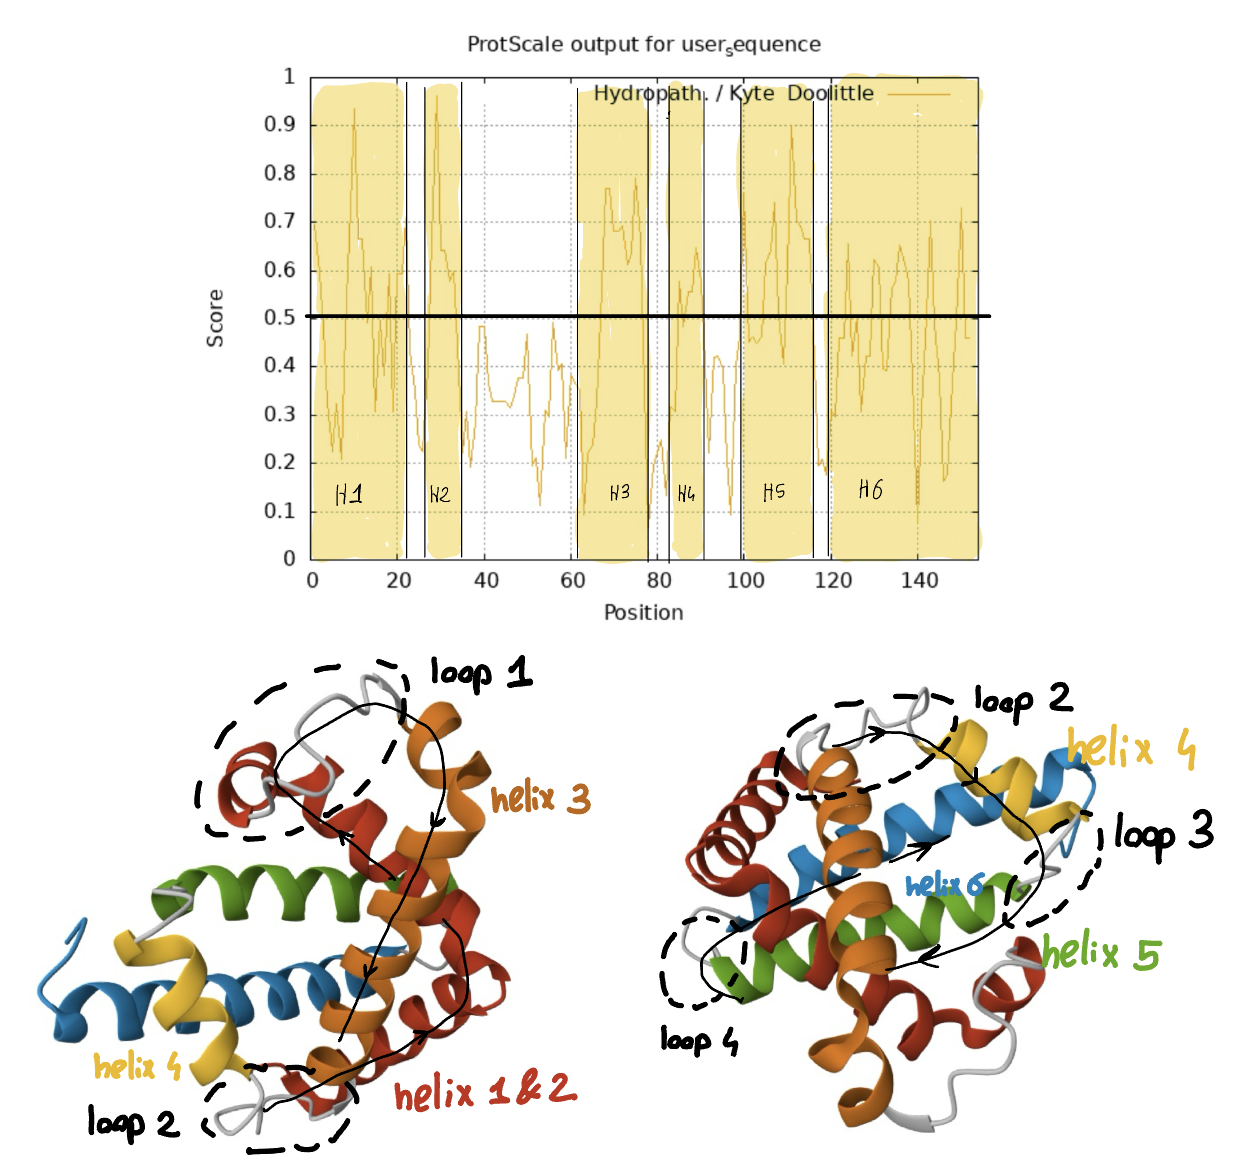
\includegraphics[width=0.6\linewidth]{slides/sequence_based_predictions/mioglobin_structure.png}
    \caption{As a quick exercise, I visualized the structure of myoglobin using the built in visualizer of PDB. To set a 
    custom coloring to your selection: i) open selection menu, ii) set coloring $\rightarrow$ miscellaneous $\rightarrow$ uniform, ii) open representation menu, color theme $\rightarrow$ value.
    The KD plot shows clearly that there are six helices in the structure, and you are able to detect from it quite precisely when they start and end!}
\end{figure}

\begin{figure}[h!]
    \centering
    \includegraphics[width=0.5\linewidth]{slides/sequence_based_predictions/helical_wheel.png}
    \caption{An example of an amino acid sequence plotted on a helical wheel. Aliphatic residues are shown as blue squares, polar or negatively charged residues as red diamonds, and positively charged residues as black octagons.
    The plot reveals whether hydrophobic amino acids are concentrated on one side of the helix, usually with polar or hydrophilic amino acids on the other. This arrangement is common in alpha helices within globular proteins, where one face of the helix is oriented
     toward the hydrophobic core and one face is oriented toward the solvent-exposed surface. (\textit{Wikipedia}) }
\end{figure}

To check for the robustness of the features, you should also check properties that are \textit{related, but not exaclty super-imposable} to hydrophobicity. For example:
\begin{itemize}
    \item polarity;
    \item $\%$ buried residues (Janin scale): based on known protein structure, where people calculated the faction of each aminoacid
    found in the exterior of the protein (exposed) versus the interior (buried);
    \item $\%$ accessible residues, similarly.
    \item bulkiness,
\end{itemize}


To summarize what we have learned:
\begin{itemize}
   \item  Learning from physico-chemical features gives the most robust predictions for proteins
\item You need to select orthogonal features, with the most relevant window sizes, which may differ between features
\item The predictions using these features will be less dataset dependent
\item The predictions using these features will be relevant \textbf{always}, in contrast to incorporation of evolutionary data (like AlphaFold)
\end{itemize}
\subsection{Using amino-acid statistics}
Now we see some methods that use pure statistics to predict the likelihood that some parts of the sequence will organize as helix, beta sheet or random coils. 
The principle is very simple: people assembled the data of known structures and computed, for each aminoacid, the probability to found it i) in an exposed helix, ii) in a
inner helix, iii) in a beta region, iv) in a coil. They interpret these probabilities as a measure of the tendence or propensity of residues in forming the various types of
secondary structures. There are softwares available online where you can simply paste the sequence. A smart move is to compare the prediction of secondary structure
given by these kind of softwares with also the \textbf{propensity to disorder}. it's an interesting thing to, to get out both information simultaneously. How much not only how much the structure wants to be a helix or beta, but how much the structure wants to be ordered, okay. So that's, that's another aspect that you may incorporate.
A software is GOR$4$:

\begin{verbatim}
    https://npsa-prabi.ibcp.fr/cgi-bin/npsa_automat.pl?page=/NPSA/npsa_gor4.html
\end{verbatim}

The very important thing to keep in mind is that these are \textit{probabilities}. Some parts of the sequence may have a strong preference for one particular 
secondary structure over the others. But many other times, the probabilities are \textit{comparable}: there is a considerable probability for more than one
structure. This is super important for biology and is being recognized more and more these days. As we already said over and over, proteins
are conformational ensembles! In the field, we call \textbf{chamaleons} those proteins that can display totally different structures.


\paragraph{Human Prion Diseases}

\begin{figure}[h!]
    \centering
    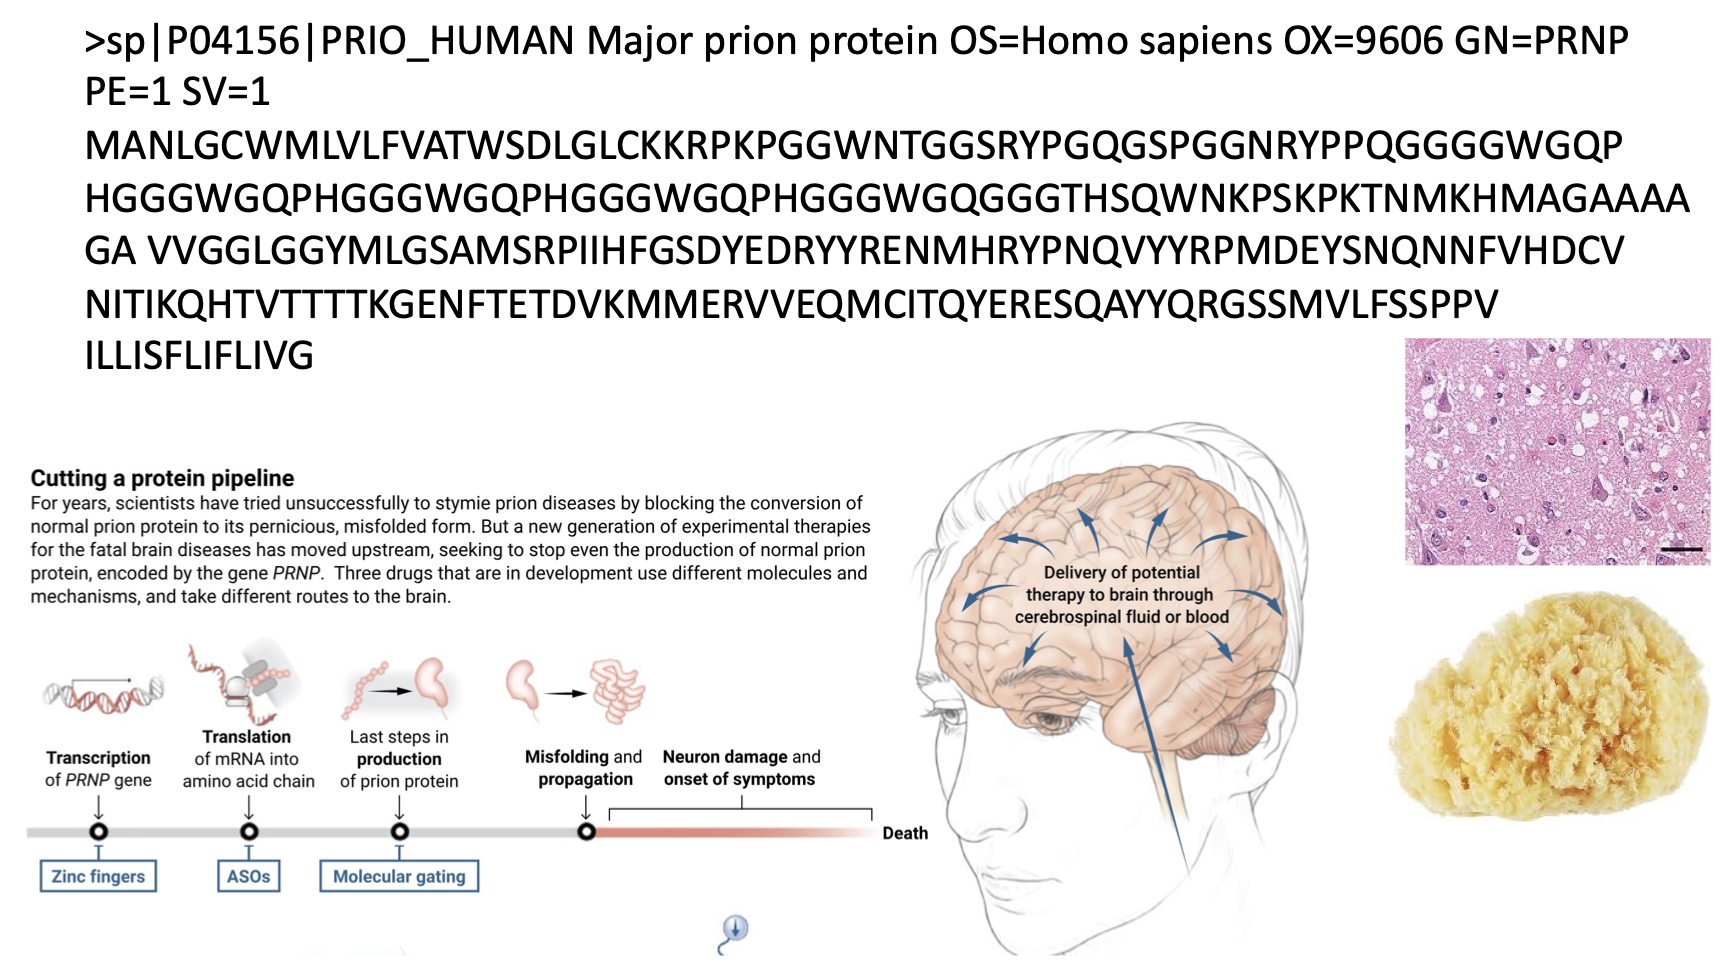
\includegraphics[width=0.55\linewidth]{slides/sequence_based_predictions/prion_diseases.png}
    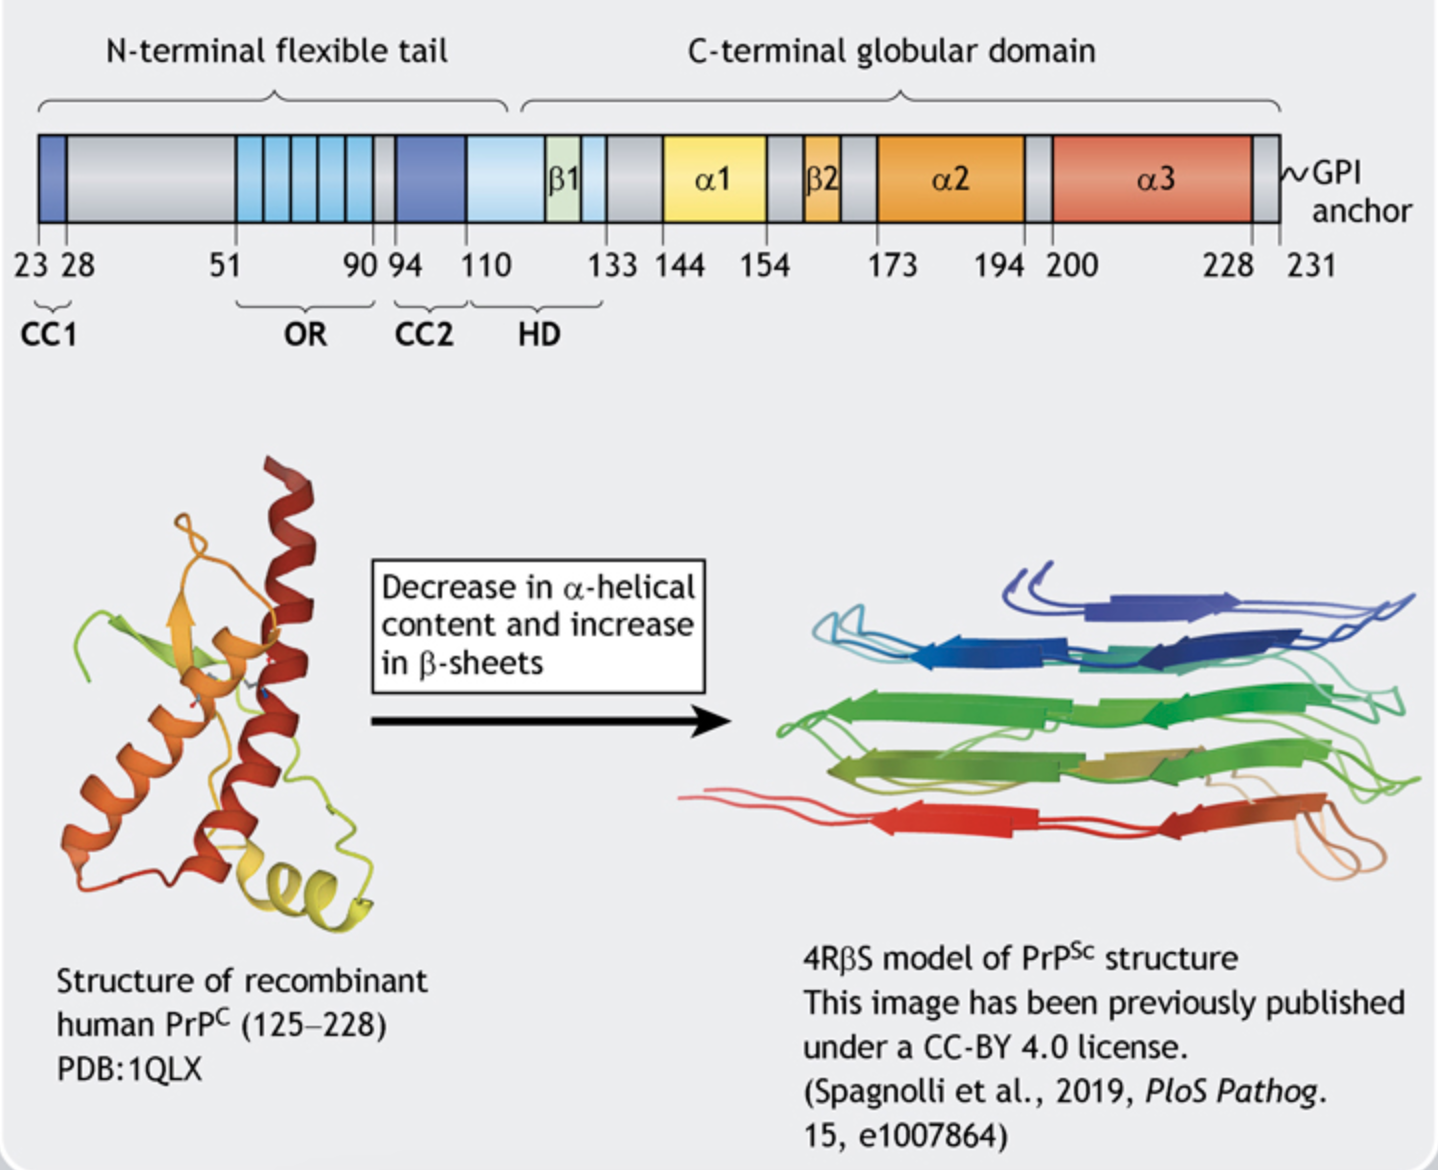
\includegraphics[width=0.4\linewidth]{slides/sequence_based_predictions/prion_aggregates.png}
    \caption{The Normal Form (PrPC): Mostly alpha-helical and soluble. The Disease Form (PrP Sc): It flips its structure to become mostly Beta-sheets. The "Infection": When a Beta-form prion touches a normal Alpha-form protein, it "convinces" (catalyzes) the Alpha-form to flip into a Beta-form. This is the "protein-based inheritance": it’s an infection without DNA or a virus.}
\end{figure}

A prion is a misfolded protein that induces folding problems in normal variants of the same protein, leading to cellular death. 
Prions are responsible for prion diseases, which are fatal and transmissible neurodegenerative diseases affecting animals including humans. 
These proteins can misfold sporadically, due to genetic mutations, \textbf{or by exposure to an already misfolded protein, leading to an abnormal three-dimensional structure that can propagate 
misfolding in other proteins} (spreading of contagion!!) (\textit{Wikipedia}). The term prion comes from "proteinaceous infectious particle". Unlike other infectious agents such as viruses, bacteria, and fungi, prions do not contain nucleic acids (DNA or RNA). 
Prions are mainly twisted isoforms of the major prion protein (PrP), a naturally occurring protein with an \textbf{uncertain} function. 
They are the hypothesized cause of various diseases, including  bovine spongiform encephalopathy (BSE) in cattle (mad cow disease), 
and Creutzfeldt–Jakob disease (CJD) in humans.  I mean you can play around with the prion protein, \textbf{you can even do a full analysis of the prion protein that can be your project}. These are super, super interesting things. 
Maybe you find something, maybe you win a million dollar not from me but from a pharmaceutical company. you had seen the prion protein structure and if you had seen the prion protein predictions, they are all helical. But when they make the disease, they are all beta. So this is already an interesting problem. This is not even one million dollar, this is probably a ten million dollar problem. Uh it has not been solved, it's for you. Uh why the helix is at a certain point changing to this uh beta and why it remains stable, that we know. But what is the role of these disordered regions, whatever, we don't know. We don't know. Uh millions and millions of dollars are invested into this, in particular since the, this, uh mad cow disease broke out in, in the UK, I, I think it was late 90s if I well recall, okay. And uh so it's not, it's, it's, it's not solved. This is like a secondary structure prediction problem that's more, uh more difficult. 
I cited here one paper you can ask from me. I mean there was this very clever biophysicist from New York who, who analyzed or collected these chameleon sequences. It seems that those proteins that aggregate also have this chameleon property.
This is for example one possible research project you can take up. Which chameleon sequences tend to form amyloids, lipid droplets, which are associated in disease? It's a pretty difficult problem. 
I would say you can, even more try to see what kind of sequences form chameleons, why do they form chameleons. It's an extremely difficult questions. 


\paragraph{Sequence similarity corresponds to structure similarity? The Paracelsus challenge }


\section{Sequence-based prediction of evolutionary links}
\paragraph{Motivation}


\subsection{Global Alignment: the Needleman-Wunsch algorithm}

\subsection{Local Alignment: the Smith-Waterman algorithm}

\subsection{Multi-Sequence Alignment (MSA)}